\noindent The  MMDP model proposed in the previous section results
in a very large search space even for small-sized problems. For
example, with 8 responders and 17 tasks in a 50$\times$55 grid, the
number of possible states is more than $2\times 10^{400}$.
Therefore, it is practically impossible to compute the optimal
solution. In such cases, it is therefore better to consider
approximate solution approaches that result in high quality
allocations.  The point of departure for our approximate solution
comes from the observations that, when making a decision, the
responders first need to {\em cooperatively} select a task to form
a team with others (i.e., agree on who will do what), and they can
{\em independently} compute the best path to the task. In our
planning algorithm, we use this observation to decompose the
decision-making process into a hierarchical structure with two
levels:
\begin{itemize}
  \itemsep=-2pt
  \item At the top level, a task allocation algorithm is run for
      the whole team to assign the best task to each responder
      given the current state of the world.
  \item At the bottom level, given a task, a path planning
      algorithm is run for each responder to find the best path
      to the task from his or her current location.
\end{itemize}

Furthermore, not all states are relevant to the problem (e.g., if a
responder gets injured, he or she is incapable of doing any task in
the future and therefore his or her states are irrelevant to other
responders) and we only need to consider the reachable states given
the current global state $S$ of the problem. Hence, given the
current state, we compute the policy online only for reachable
states. This saves a lot of computation because the size of the
reachable states is usually much smaller than the overall state
space. For example, given the current location of a responder, the
one-step reachable locations are the 8 neighbouring locations plus
the current locations, which are 9 locations out of the
50$\times$55 grid. Jointly, the reduction will be huge, which is
$9^8$ vs. $(50\times 55)^8$ for 8 responders. Another advantage of
online planning is that it allows us to tweak the model as more
information is obtained or unexpected events happen. For example,
if the wind speed increases or the direction of wind increases, the
uncertainty about the radioactive cloud may increase. If a
responder becomes tired, the outcome of his or her actions may be
liable to more uncertainty.

The main process of our online hierarchical planning algorithm is
outlined in Algorithm~\ref{alg:coordination}. The following
sections will describe the procedures of each level in more detail.

\begin{algorithm}[t]
  \caption{Team Coordination}\small
  \label{alg:coordination}
  \Indm
  \KwIn{the MMDP model and the current state $s$.}
  \KwOut{the best joint action $\vec{a}$.}
  \Indp\BlankLine
  \tcp{The task planning}
  $\{ t_i \} \gets$ compute the best task for each responder $i\in I$ \;
  \ForEach{$i\in I$} {
    \tcp{The path planning}
    $a_i \gets$ compute the best path to task $t_i$ \;
  }
  \Return{$\vec{a}$}
\end{algorithm}

\subsection{Task Allocation}
\label{sec:taskplanning}

\noindent As described in Section \ref{sec:model}, each responder
$p_i$ has a specific role $r_i \in Roles$ to determine which task
he or she can perform and  a task $t$ can only be completed by a
team of responders with the required roles $Roles(t)$. If, at some
point in the execution of a plan, a responder $p_i$ is incapable of
performing a task (e.g., because she is tired or suffered a high
radiation does), he or she will be removed from the set of
responders under consideration that is $I = I \setminus p_i$ if
$pi$. This information can be obtained from the state $s \in S$.
When a task is completed by a chosen coalition, the task is simply
removed from the set, that is $T = T\setminus t_k$ if $t_k$ has
been completed.

Now, in order to capture the efficiency of groupings of responders
at performing tasks, we define the notion of a coalition $C$ as a
subset of responders, that is, $C \subseteq I$.\footnote{Here
coalitions are not considered in the game-theoretic sense as all
agents and coalitions aim to maximise the global objective.} Thus,
we can identify all possible coalitions $\{ C_{jk} \}$ for each
task $t_j$ where $\{r_i | p_i \in C_{jk}\} = Roles(t_j)$.
Crucially, we define the value of a coalition $v(C_{jk})$ that
reflects the level of performance of a coalition $C_k$ in
performing task $t_k$.  Then, the goal of task allocation algorithm
is to assign a task to each coalition that maximises the overall
team performance given the current state $s$, i.e., $\sum_{j=1}^m
v(C_j)$ where $C_j$ is a coalition for task $t_j$ and $\{ C_1,
\cdots, C_m \}$ is a {\em partition} of $I$ ($\forall j\neq j', C_j
\bigcap C_{j'} = \emptyset$ and $\bigcup_{j=1}^m C_j=I$). In what
follows, we first detail the procedure to compute the value of all
coalitions that are valid in a given state and then proceed to
detail the main algorithm to allocate tasks. Note that these
algorithms take into account the uncertainties captured by the
MMDP.


\subsubsection{Coalition Value Calculation}
The computation of values  $v(C_{jk})$ for each coalition $C_{jk}$
is challenging because not all tasks can be completed by one
allocation (there are usually more tasks than responders) and the
policy after completing task $t_j$ must be computed as well and
this is time-consuming. Here, we propose to estimate the value
through several simulations. This is much cheaper computationally
because we do not need to compute the complete policy in order to
come up with a good estimate of the value of the coalition.
According to the central limit theorem, as long as the number of
simulations is sufficient large, the estimated value will converge
to the true coalition value. The main process is outlined in
Algorithm~\ref{alg:taskplanning}.
\begin{algorithm}[htbp]\small
  \caption{Coalition Value Calculation}
  \label{alg:taskplanning}
  \Indm
  \KwIn{the current state $s$,
  a set of unfinished tasks $T$,
  and a set of free responders $I$.}
  \KwOut{a task assignment for all responders.}
  \Indp\BlankLine
  $\{ C_{jk} \} \gets$ compute all possible coalitions of $I$ for
  $T$ \;
  \ForEach{$C_{jk} \in \{C_{jk}\}$}{
    \tcp{The $N$ trial simulations}
    \For{$i=1$ \KwTo $N$}{
        $(r, s') \gets$ simulate the process with the starting state $s$
        until task $k$ is completed by the responders in $C_{jk}$ \;
        \If{$s'$ is a terminal state} {
            $v_i(C_{jk}) \gets r$ \;
        } \Else {
            $V(s') \gets$ estimate the value of $s'$ with MCTS \;
            $v_i(C_{jk}) \gets r + \gamma V(s')$ \;
        }
    }
    $v(C_{jk}) \gets \frac{1}{N} \sum_{i=1}^{N} v_i(C_{jk})$ \;
  }
  \Return the task assignment computed by Equation~\ref{eq:cf}
\end{algorithm}

In each simulation of Algorithm~\ref{alg:taskplanning}, we first
assign the responders in $C_{jk}$ to task $t_j$ and run the
simulator starting from the current state $s$ (Line 4). After task
$t_j$ is completed, the simulator returns the sum of the rewards
$r$ and the new state $s'$ (Line 4). If all the responders in
$C_{jk}$ are incapable of doing other tasks (e.g., having received
too high a radioactive dose), the simulation is terminated (Line
5). Otherwise, we estimate the expected value of $s'$ using
Monte-Carlo Tree Search (MCTS) (Line 8), which provides good
tradeoff between exploitation and exploration of the policy space
and has been shown to be efficient for large MDPs~\cite{?}. After
$N$ simulations, the averaged value is returned as an approximation
of the coalition value (Line 10).

The basic idea of MCTS is to maintain a search tree where each node
is associated with a state $s$ and each branch is a task assignment
for all responders. To implement MCTS, the main step is to compute
an assignment for the free responders (a responder is free when he
or she is capable of doing tasks but not assigned to any task) at
each node of the search tree. This can be computed by
Equation~\ref{eq:cf} using the coalition values estimated by the
UCT heuristic~\cite{?}:
\begin{equation}
  v(C_{jk}) = \overline{v(C_{jk})} + c\sqrt{\frac{2N(s)}{N(s, C_{jk})}}
\end{equation}
where $\overline{v(C_{jk})}$ is the averaged value of coalition
$C_{jk}$ at state $s$ so far, $c$ is a tradeoff constant, $N(s)$ is
the visiting frequency of state $s$, and $N(s, C_{jk})$ is the
frequency that coalition $C_{jk}$ has been selected at state $s$.
Intuitively, if a coalition $C_{jk}$ has bigger averaged value
$\overline{v(C_{jk})}$ or is rarely selected ($N(s, C_{jk})$ is
smaller), it has higher chance to be selected in the next visit of
the tree node.

As we assume that the role of a responder and the role requirements
of each task is static, we can compute all possible coalition
values offline and therefore, in the online phase, we only need to
filter out the coalitions for completed tasks and those containing
incapacitated responders to compute the coalition set $\{ C_{jk}
\}$.

\subsubsection{Coalitional Task Allocation}
Given the coalition values computed above, we then solve the following
optimisation problem to find the best solution:
\begin{equation}
  \begin{array}{lll}
    \max\limits_{x_{jk}} & \sum_{j, k} x_{jk} \cdot v(C_{jk}) & \\[2pt]
    \mbox{s.t.} & x_{jk} \in \{0, 1\} & \\[2pt]
    & \forall j, \sum_{k} x_{jk} \leq 1 & \mbox{(i)} \\[2pt]
    & \forall i, \sum_{j, k} \delta_i(C_{jk}) \leq 1 & \mbox{(ii)}
  \end{array}
  \label{eq:cf}
\end{equation}
where $x_{jk}$ is the boolean variable to indicate whether
coalition $C_{jk}$ is selected for task $t_j$ or not, $v(C_{jk})$
is the characteristic function for coalition $C_{jk}$, and
$\delta_i(C_{jk}) = 1$ if responder $p_i\in C_{jk}$ and 0
otherwise. In the optimisation, Constraint (i) ensures that a task
$t_j$ is allocated at most to only one coalition (a task does not
need more than one group of responders). Constraint (ii) ensures
that a responder $p_i$ is assigned to only one task (a responder
cannot do more than one task at the same time). This is a standard
MILP that can be efficiently solved  using standard solvers such as
IBM ILOG's CPLEX.

\subsubsection{Adapting to Responders}
One main advantage of our approach is that it can easily
incorporate the preferences of the responders. For example, if a
responder rejects  a task allocated to it by the planning agent, we
simply filter out the coalitions for the task that contain the
responder. By so doing, the responder will not be assigned to the
task. Moreover, if a responder prefers to do the tasks with another
responder, we can increase the weights of the coalitions that
contain them in Equation~\ref{eq:cf} (By default, all coalitions
have identical weights of 1.0). Thus, our approach is adaptive to
various preferences of human responders. In particular, we show how
the adaptive capability of our algorithm is used in AtomicOrchid in
a real-world deployment (in Section \ref{sec:evaluation}) Next we
show how the path of each responder is computed taking into account
real-world uncertainties.

\subsection{Path planning}
\label{sec:pathplanning}

\noindent In the path planning phase, we compute the best path for
a responder to her assigned task. This phase is stochastic as there
are uncertainties in the radioactive cloud and the responders'
actions. We model this problem as a single-agent MDP that can be
defined as a tuple, $\mathcal{M}_i = \langle S_i, A_i, P_i, R_i
\rangle$, where: $S_i = S_r \times S_{p_i}$ is the state space. In
this level, responder $p_i$ only need to consider the states of the
radioactive cloud $S_r$ and his or her own states $S_{p_i}$ in the
MMDP. $A_i$ is the set of $p_i$'s actions. In this level, responder
$p_i$ only need to consider her moving actions. $P_i = P_r \times
P_{p_i}$ is the transition function. In this level, responder $p_i$
only need to consider the spreading of the radioactive cloud $P_r$
and the changes of his or her locations and health levels when
moving in the filed $P_{p_i}$, which are defined earlier in the
MMDP. $R_i$ is the reward function. At this level, responder $p_i$
only needs to consider the cost of moving to a task and the penalty
of receiving high radiation doses.

This is a typical MDP that can be solved by many state-of-the-art
MDP solvers~\cite{?}. We choose the Real-Time Dynamic Programming
(RTDP)~\cite{?} approach because it particularly fits  our problem,
that is, a goal-directed MDP with large number of states. Instead
of exploring the whole state space, RTDP only visits the states
that are reachable from the initial state $s^0$ (the start location
of the responder). In each iteration of RTDP, we first compute the
$Q$ value for each action and select the best action for the
responder. Then, we update the value function and simulate the next
state. This process repeats until the goal state is reached. If the
goal is not reached, we assume there does not exist a path between
the start location of the responder and the location of the task
(either there are obstacles on the path or the responder will be
killed by the radioactivity on the road).
%\begin{algorithm}[htbp]
%  \caption{Path Planning}
%  \label{alg:pathplanning}
%  \Indm
%  \KwIn{the starting state $s^0$ and the goal state $s^g$.}
%  \KwOut{a path from the starting location to the goal.}
%  \Indp\BlankLine
%  \While{not out of time}{
%      $s \gets s^0$ \;
%      \Repeat{$s = s^g$}{
%        \ForEach{$a\in A_i$}{
%            $Q(s, a) \gets R_i(s, a) + \sum_{s'\in S_i} P_i(s'|s, a)
%            V(s')$ \;
%        }
%        $a \gets \arg\max_{a'\in A_i} Q(s, a')$ \;
%        $V(s) \gets Q(s, a)$ \;
%        $s' \sim P_i(s'|s, a)$ \;
%        $s \gets s'$ \;
%      }
%  }
%  \Return{$Q$}
%\end{algorithm}

There are several techniques we use to speed up the convergency of
RTDP. In our problem, the terrain of the field is static. Thus, we
can initialize the value function $V(s)$ using the cost of the
shortest path between the current location to the task location on
the map, which can be computed offline without considering the
radioactive cloud. This helps RTDP quickly navigate among the
obstacles (e.g., buildings, water pools, blocked roads) without
getting trapped in dead-ends during the search. Another speed up is
also possible if, when traversing the reachable states (i.e.,
$s'\in S_i$ in Line 4), we only consider the responder's current
location and the neighbouring points, since $P_i(s'|s,a) = 0$ for
other points. This will further speed up the algorithm where the
main bottleneck is the huge state space.

\subsection{Simulation results}

\begin{figure}[htbp]
  \centering
  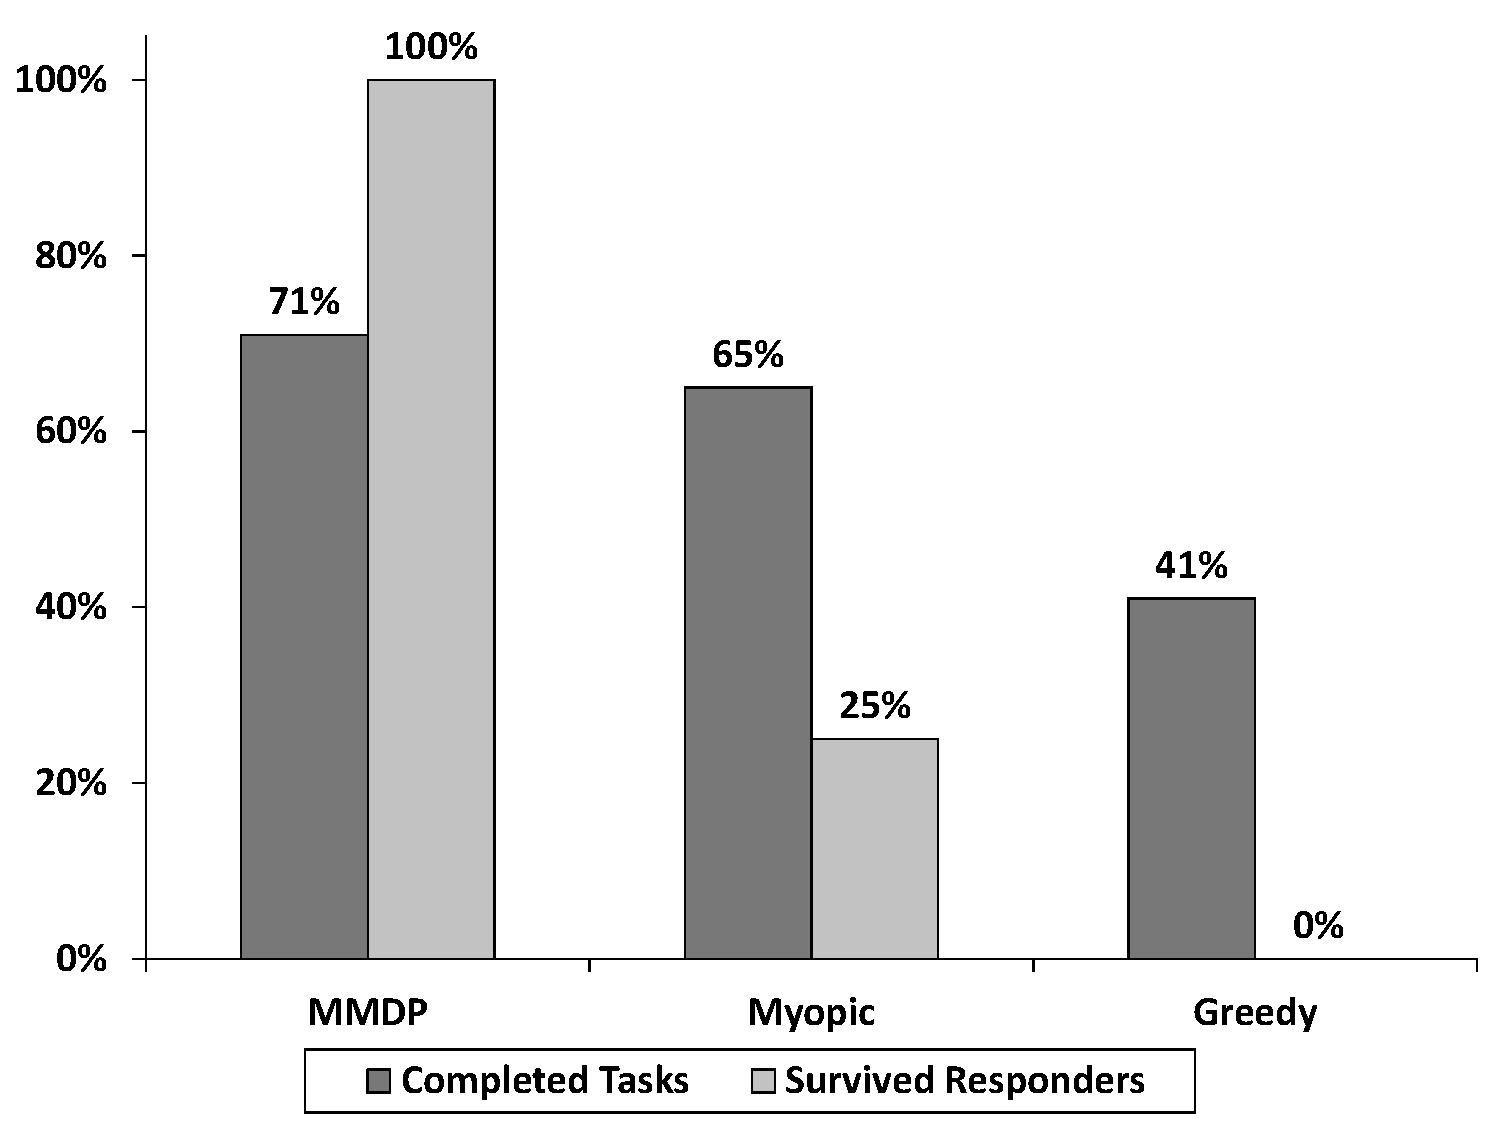
\includegraphics[width=0.8\linewidth]{simulation}
  \caption{Experimental results for the MMDP, myopic, greedy
  algorithms in simulation.}
  \label{fig:simulation}
\end{figure}

\noindent To test the performance of our algorithm, we compare it
with a greedy and a myopic method for task planning using a
simulator. For each method, we use our path planning algorithm to
compute the path for each responder so that they can reach the task
location as fast as possible. In the greedy method, the responders
are uncoordinated and select the closest tasks that they can do. In
the myopic method, the responders are coordinated to select the
tasks but have no lookahead for the future tasks.
Figure~\ref{fig:simulation} shows the results for a problem with 17
tasks and 8 responders on a 50$\times$55 grid. As we can see, our
MMDP algorithm can complete more tasks than the myopic and greedy
methods. More importantly, our algorithm can guarantee the safety
of the responders while in the myopic method, only 25\% of the
responders are survived and in the greedy method all responders are
killed by the radioactive cloud. More extensive evaluations are
beyond the scope of this paper as the focus is on the use of the
algorithm in a real-world deployment to test how humans take up
advice computed in sophisticated ways by an agent-based planner.

%(\textbf{Feng: just provide a graph depicting the performance of
%the algorithm compared to greedy and say more extensive evaluations
%are beyond the scope of this paper as the focus is on the use of
%the algorithm in a real-world deployment to test how humans take up
%advice computed in sophisticated ways by an agent-based planner)}.
